The explicit expressions for the flow field are shown in \eqref{eq:explicit_u_h} and \eqref{eq:explicit_v_h}. The flow field within the glacier can be computed by evaluating these equations on grid points within the glacier. The derivative in \eqref{eq:explicit_v_h} is approximated using central differences. Forward and backwards differences are used on the boundaries of the grid.

The stationary glacier for a given accumulation rate is found using the method described in \red{reference to relevant section or equation}.

\iffalse
\begin{figure}%
    \centering
    \subfloat[Arbitrary accumulation rate]{{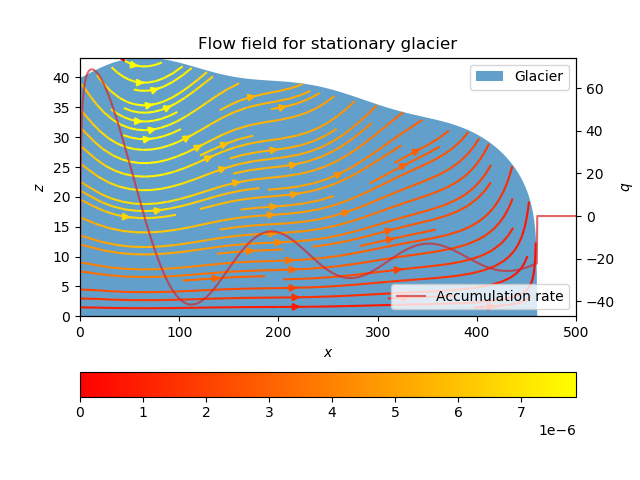
\includegraphics[width=5cm]{report/images/flow_field_arbitrary_production.png}}}%
    \qquad
    \subfloat[Accumulation rate as specified in \red{relevant equation} ]{{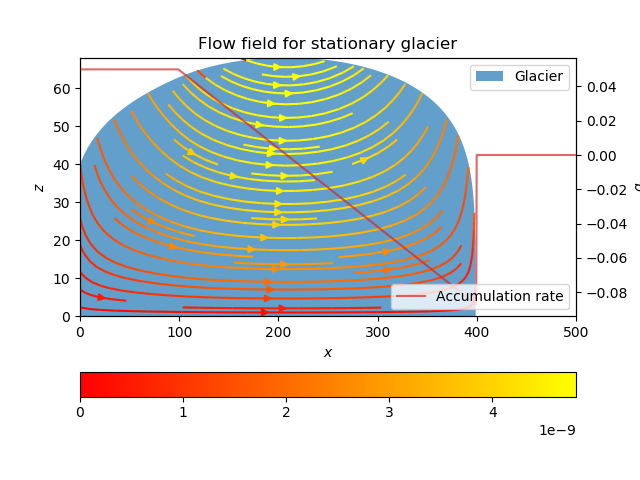
\includegraphics[width=5cm]{report/images/flow_field_linear_production.png}}}{\label{fig:linear}%
    \caption{Stationary glaciers with height on left axis, accumulation rate on right axis and stream lines for the internal flow field}\label{fig:arbitrary}%
    \label{fig:example}%
\end{figure}
\fi

\begin{figure}
    \centering
    \begin{subfigure}[b]{0.4\textwidth}
        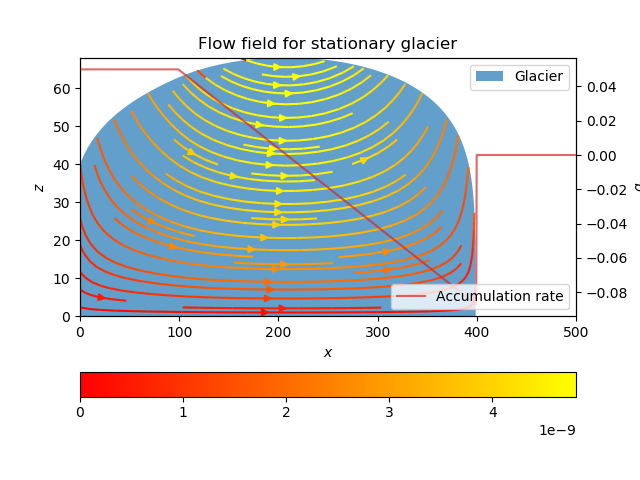
\includegraphics[width=\textwidth]{report/images/flow_field_linear_production.png}
        \caption{Accumulation rate as specified in \red{a}}
        \label{fig:linear}
    \end{subfigure}
    \begin{subfigure}[b]{0.4\textwidth}
        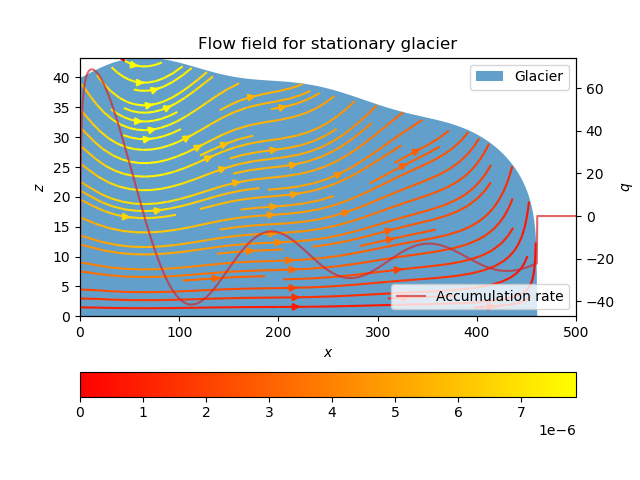
\includegraphics[width=\textwidth]{report/images/flow_field_arbitrary_production.png}
        \caption{Arbitrary accumulation rate}
        \label{fig:arbitrary}
    \end{subfigure}
    \caption{Stationary glaciers with height on left axis, accumulation rate on right axis and stream lines for the internal flow field}\label{fig:animals}
\end{figure}

The flow field for the production rate $q(x) = 5\sin(\frac{x}{25})\frac{1}{2(x + 1)} - 0.01$ is shown in figure \ref{fig:arbitrary}.

The flow field for a production rate as shown in \red{Description of accumulation rate} is shown in figure \ref{fig:linear}.